\subsection{观测阶段性能剖析}\label{sec:observation}

观测阶段（Observation）对应主循环中的 \texttt{robot.get\_observation()}。
在本文的 SO-101 实验配置中，一次 observation 由两类数据组成：
两路 OpenCV 摄像头图像，以及一个 follower 机械臂的 6 个舵机当前位置。
其中两路摄像头分别为 \texttt{handeye} 和 \texttt{fixed}，分辨率均为
640$\times$360；舵机状态来自 6 个 STS3215 舵机的
\texttt{Present\_Position} 寄存器。

从代码结构看，SO-101 follower 的观测函数先同步读取 6 个舵机位置，
随后遍历两路相机，取回后台线程已经预取的图像。
这意味着观测阶段（Observation，实验字段记为 \texttt{obs}）并不是单一 I/O，
而是“舵机同步读 + 两路相机异步取帧”的组合。
舵机读取与执行阶段共用同一条 \texttt{/dev/ttyACM0} 半双工总线，
协议和内核路径高度重合，
因此本节只点明其在 obs 中的位置，详细分析放在 \S\ref{sec:execution}。

\subsubsection{摄像头异步读取机制}

LeRobot 的 OpenCV 相机并不是在主线程里每次直接阻塞读取硬件帧。
每个相机对象内部维护一个后台读线程：只要没有收到停止信号，
它就循环调用 OpenCV 读取摄像头，把最新图像写入共享缓存，并设置帧就绪事件。
主线程中的 \texttt{async\_read()} 不再直接面对摄像头设备，
而是等待这个事件；事件到达后，它只需短暂获取锁，
从共享缓存取走最近一帧，然后清除事件标志，等待下一次更新。
这里不是两个线程互相通知：后台线程负责生产帧并设置事件，主线程负责等待事件并清除事件。

\begin{figure}[htbp]
  \centering
  \begin{tikzpicture}[
    >=Stealth,
    lane/.style={rectangle, draw=gray!70, fill=gray!5, rounded corners=2pt,
      minimum width=2.6cm, minimum height=0.8cm, align=center, font=\small},
    proc/.style={rectangle, draw=blue!60, fill=blue!8, rounded corners=2pt,
      minimum width=2.9cm, minimum height=0.75cm, align=center, font=\footnotesize},
    shared/.style={rectangle, draw=orange!70, fill=orange!10, rounded corners=2pt,
      minimum width=2.9cm, minimum height=0.75cm, align=center, font=\footnotesize},
    note/.style={font=\scriptsize, text=gray!75}
  ]
    \node[lane] (bg) at (0, 2.1) {后台相机线程};
    \node[proc, right=0.8cm of bg] (read) {OpenCV 取帧\\MJPEG 解码};
    \node[shared, right=0.8cm of read] (cache) {更新图像缓存\\短锁保护};
    \node[proc, right=0.8cm of cache] (event) {设置帧就绪事件};

    \node[lane] (main) at (0, -0.35) {主线程观测阶段};
    \node[proc, right=0.8cm of main] (wait) {等待帧就绪事件};
    \node[shared, right=0.8cm of wait] (take) {读取图像缓存\\清除事件标志};
    \node[proc, right=0.8cm of take] (return) {返回图像};

    \draw[->, thick, blue!65] (bg) -- (read);
    \draw[->, thick, blue!65] (read) -- (cache);
    \draw[->, thick, blue!65] (cache) -- (event);
    \draw[->, thick, red!65] (event.south) -- node[pos=0.30, above, note, fill=white, inner sep=0.8pt]{单向通知} (wait.north);
    \draw[->, thick, blue!65] (main) -- (wait);
    \draw[->, thick, blue!65] (wait) -- node[pos=0.50, above, note, fill=white, inner sep=0.8pt]{加锁} (take);
    \draw[->, thick, blue!65] (take) -- (return);
    \draw[->, thick, blue!65, rounded corners=8pt]
      (event.north) -- ++(0,0.55) -| node[pos=0.25, above, note]{未停止时继续循环} (read.north);
    \draw[->, dashed, thick, gray!70]
      (take.north) -- node[pos=0.45, right, note]{复位标志，不通知后台线程} (event.south);
  \end{tikzpicture}
  \caption{OpenCV 摄像头异步读取中的后台循环、单向事件通知与主线程取缓存关系}
  \label{fig:opencv-async-read}
\end{figure}

后台线程会调用 OpenCV 的读帧接口，从 V4L2 摄像头设备取出一帧，
并在用户态完成 MJPEG 解码和颜色格式整理。整理后的 RGB 图像被写入
\texttt{latest\_frame}，这个共享缓存由 \texttt{frame\_lock} 保护。
\texttt{new\_frame\_event} 只承担“帧已就绪”的单向通知作用；
主线程取走缓存帧后会复位事件标志，避免下一轮直接读到旧帧，
但这个复位动作不会反向唤醒或驱动后台相机线程。

因此，\texttt{async\_read()} 的“异步”含义是：摄像头硬件读取和 MJPEG 解码
提前在后台线程中进行，主线程在观测阶段只等待事件并读取最近一帧。
如果后台线程已经准备好图像，主线程很快返回；如果主线程跑得比相机帧率更快，
则会在等待新帧事件时阻塞。

\subsubsection{是否进入内核}

摄像头路径中有三类等待，需要区分其含义。

\begin{center}
\small
\begin{tabularx}{\textwidth}{>{\raggedright\arraybackslash}p{0.22\textwidth}
  >{\raggedright\arraybackslash}p{0.28\textwidth}
  >{\raggedright\arraybackslash}X}
  \toprule
  位置 & 是否可能进入内核 & 含义 \\
  \midrule
  主线程等新帧事件 & 可能进入内核 &
  线程同步等待。对应 \texttt{new\_frame\_event.wait()}，
  主线程等后台相机线程把新帧准备好 \\
  主线程取缓存帧 & 通常不进入内核 &
  短锁保护。对应 \texttt{frame\_lock}，
  只是在读写 \texttt{latest\_frame} 时避免两个线程同时改同一块缓存 \\
  OpenCV 后台线程取帧 & 会进入内核 &
  设备可读等待。后台线程通过 \texttt{select()} 等待 V4L2 摄像头有帧可取，
  随后再执行出队操作取得该帧 \\
  \bottomrule
\end{tabularx}
\end{center}

也就是说，主线程的 \texttt{async\_read()} 主要是在等 Python 线程同步事件；
真正深入 V4L2、USB 摄像头驱动和 videobuf2 队列的是后台读线程。
这也是为什么主线程观测耗时可能只有毫秒级，而摄像头后台线程的
\texttt{pselect6} 等待会接近 30 fps 的帧间隔。

\subsubsection{OpenCV 到内核的边界}

论文正文不展开完整源码栈，只保留性能分析需要的边界关系：
后台相机线程首先进入 OpenCV 的 \texttt{VideoCapture}，随后通过 glibc
发起 V4L2 相关系统调用，最终进入 Linux 的 V4L2、UVC 和 videobuf2 队列。

\begin{figure}[htbp]
  \centering
  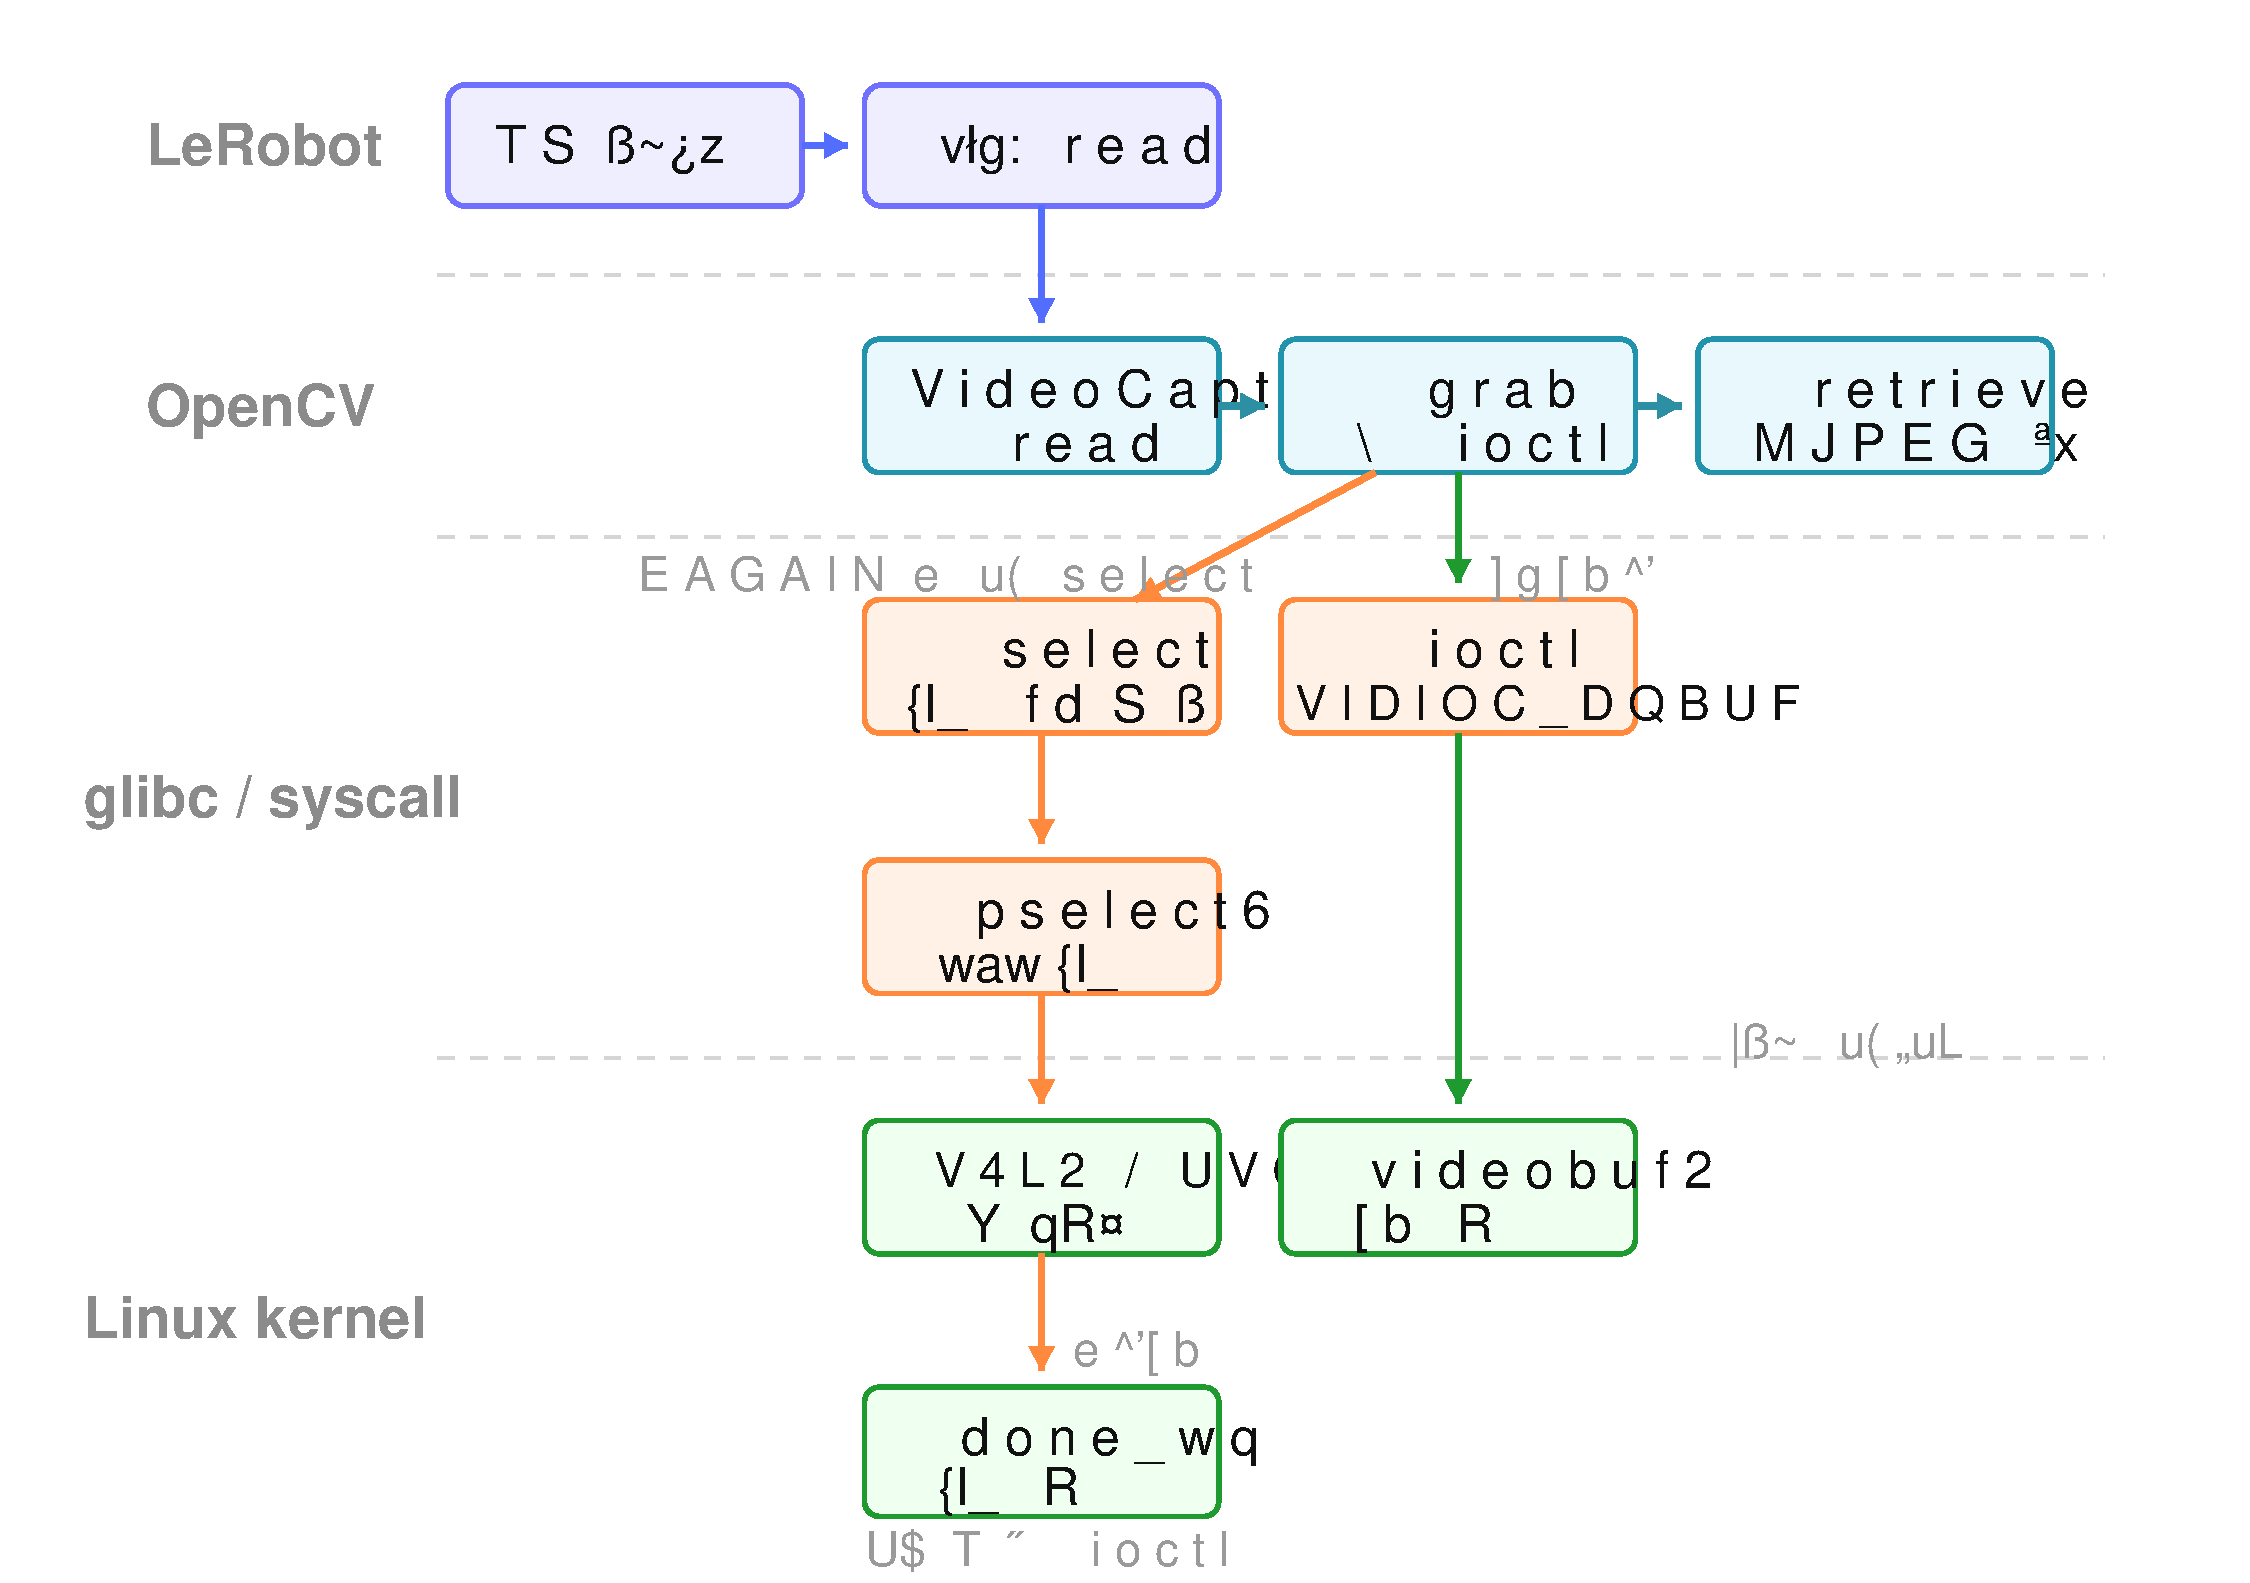
\includegraphics[width=0.98\textwidth]{3_性能分析/image/opencv_v4l2_callstack.pdf}
  \caption{OpenCV 摄像头后台线程从用户态到 V4L2 内核队列的关键路径}
  \label{fig:opencv-v4l2-callstack}
\end{figure}

图~\ref{fig:opencv-v4l2-callstack} 中有两条需要区分的路径：
等待设备可读通常发生在 \texttt{select()} / \texttt{pselect6} 一类调用上；
真正取出已完成图像缓冲区时，OpenCV 使用 \texttt{VIDIOC\_DQBUF} 将一个已经由驱动填好的
V4L2 buffer 从完成队列中出队。

需要注意的是，\texttt{VIDIOC\_DQBUF} 并不是把整帧像素从内核重新拷贝一遍。
在当前 OpenCV V4L2 路径中，摄像头 buffer 通过 mmap 暴露给用户态；
出队操作主要返回 buffer 的编号、有效字节数和时间戳等元数据。
MJPEG 到 BGR 图像的解码仍然发生在用户态 OpenCV/libjpeg 中，
这部分才是 ARM CPU 上摄像头链路中更明显的计算开销。

\subsubsection{时间剖析}

在 30 fps 摄像头配置下，单路摄像头物理帧间隔约为 33.3 ms。
实测中，后台线程在 \texttt{pselect6} 或 V4L2 等待路径中阻塞约 23--32 ms，
符合摄像头帧率上限；MJPEG 解码仍在用户态 OpenCV/libjpeg 中完成，
在 ARM CPU 上属于摄像头链路的主要计算开销。
由于 LeRobot 采用后台预取，主线程观测阶段看到的是“取缓存帧”的时间，
而不是完整的摄像头端到端采集时间。
因此，主线程通常不会被摄像头硬件读取、V4L2 等待或 MJPEG 解码直接阻塞；
这些耗时主要由后台相机线程承担。主线程只有在请求图像时后台线程尚未准备好新帧，
才会短暂等待 \texttt{new\_frame\_event}，随后只是持锁读取最近缓存帧。
